% this is source code for one of the sessions in Digital Skills for Research Workshop (EMTTI, University of Wolverhampton)
% March 2022, Maria Kunilovskaya (mkunilovskaya@gmail.com)

%--------------------
% Preamble

% Declare the type of document
% -------------------

\documentclass[a4paper,12pt]{article} % other options: [,twocolumn,leqno]{report, book, beamer} 

%--------------------
% Import packages
% -------------------

\usepackage[utf8]{inputenc}  % specify the encoding
\usepackage{hyperref} % allow cross-referencing
\usepackage{geometry} % set the layout
\geometry{
	a4paper,
	total={170mm,257mm},
	left=20mm,
	top=20mm,
}
\usepackage{xcolor} % alow color for text
\usepackage{tcolorbox} % make boxes
\usepackage{multicol} % columns

\usepackage{graphicx} % insert pictures
%\graphicspath{{images/}{pics/}}  % from folders with .png, .jpj, .gif, .eps

%--------------------
% Define new commands and settings
% -------------------

% TeX logo as defined by Donald Knuth in the TeXbook (1984)
\def\TeX{{\rm T\kern-.1667em\lower.5ex\hbox{E}\kern-.125emX }}
\newcommand{\llogo}{\LaTeX }

\setlength\parindent{0pt} % don't indent new paragraphs

%--------------------
% Setup the title of the document
% -------------------

\title{\vspace{-4em} Digital Skills for Research}
\author{Maria Kunilovskaya\thanks{thanks to the RGCL for the opportunity to brush up and systematise these}}
\date{02 March - 25 March, 2022}

\begin{document}
	
%remove numbering from the first page
\clearpage\maketitle
\thispagestyle{empty}	
\maketitle

\vspace{-2em}

\section{{\color{red}\TeX and \LaTeX}}

\subsection{Week 1. Setup and Start}\footnote{to compile pdfs download the necessary support files from the respective folders, not just the linked .tex}
	Session 1. Why \TeX and first doc (\href{https://canvas.wlv.ac.uk/courses/33429/files/folder/latex_mendeley_github/w1-3_latex?preview=4622172}{pdf}, \href{https://github.com/kunilovskaya/dskills_workshop/blob/main/w1_latex_basics/session1.tex}{class tex}, \href{https://github.com/kunilovskaya/dskills_workshop/blob/main/w1_latex_basics/task1.tex}{task})
		\begin{itemize}
			\item What's \TeX (distributions, editors, engines, formats, templates)
			\item Overleaf account and project
			\item First document (class, packages, layout, title, sections, margins, columns)
		\end{itemize} 
	Session 2. Text and math (\href{https://canvas.wlv.ac.uk/courses/33429/files/folder/latex_mendeley_github/w1-3_latex?preview=4623463}{pdf}, \href{https://github.com/kunilovskaya/dskills_workshop/blob/main/w1_latex_basics/session1.tex}{class tex}, \href{https://github.com/kunilovskaya/dskills_workshop/blob/main/w1_latex_basics/task2.pdf}{task})
		\begin{itemize}
			\item Text formatting
			\item Special characters
			\item Math
		\end{itemize}

\subsection*{Week 2. Environments and Customisation}
	Session 3. Tables and figures (\href{https://github.com/kunilovskaya/dskills_workshop/blob/main/w2_latex_frills/session3.tex}{class tex}, \href{https://github.com/kunilovskaya/dskills_workshop/blob/main/w2_latex_frills/task3.tex}{task})
			\begin{itemize}
				\item Environments
				\item Tables
				\item Graphics and drawing
			\end{itemize}
	Session 4. Customisation, cross-referencing and templates (\href{https://github.com/kunilovskaya/dskills_workshop/blob/main/w2_latex_frills/session4.tex}{class tex}, \href{https://github.com/kunilovskaya/dskills_workshop/blob/main/w2_latex_frills/task4.tex}{task})
			\begin{itemize}
				\item Own commands
				\item Internal and external links
				\item Templates and big projects
			\end{itemize}

\subsection*{Week 3. Beamer and Bibs}
	Session 5. Presentations and posters (\href{https://github.com/kunilovskaya/dskills_workshop/blob/main/w3_bibs_beamer/session5.tex}{class tex}, \href{https://github.com/kunilovskaya/dskills_workshop/blob/main/w3_bibs_beamer/task5.tex}{task})
	\begin{itemize}
		\item Beamer themes: layout and colour
		\item Slides-specific commands
		\item Producing posters and own .sty 
	\end{itemize}

\newpage

	Session 6. Bibliographies (\href{https://canvas.wlv.ac.uk/courses/33429/files/folder/LaTeX\%20and\%20Mendeley\%20workshop/w1-3_latex?preview=4648015}{class pdf}, \href{https://github.com/kunilovskaya/dskills_workshop/blob/main/w3_bibs_beamer/task6.tex}{task})
	\begin{itemize}
		\item Basics on referencing styles
		\item .bib files and bibliography engines
		\item Get References section
	\end{itemize}	

\section{{\color{red}Week 4. Mendeley and Github}}
	Session 7. Reference management: Mendeley (\href{}{pdf}, \href{}{task})
	\begin{itemize}
		\item Basic uses and setting up
		\item Integration (word processor, browser, project)
		\item Library use and maintenance 
		% (+ note-taking tools)
	\end{itemize}%
	Session 8. Version control and collaboration: Git and GitHub (\href{}{pdf}, \href{}{task})
	\begin{itemize}
		\item Keeping track of changes
		\item Local and remote, push and pull, auth
		\item Markdown and arranging repos
	\end{itemize}

\begin{center}
	
\begin{tcolorbox}[width=\textwidth, colback={blue!10!white}, title={\textbf{Learning strategies behind the workshop design (in the order of importance)}}, colbacktitle=blue!30!white, coltitle=black]
	\begin{itemize}
		\item distributed learning: building skills over time VS cramming all at once
		
		\begin{center}
			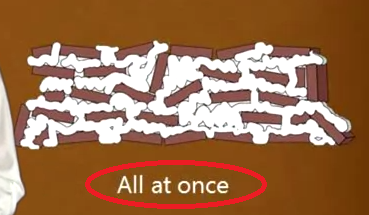
\includegraphics[width=40 mm]{pics/all at once.png} \hspace{2cm}
			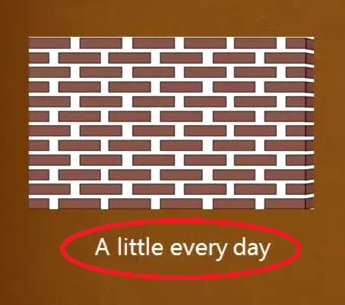
\includegraphics[width=30 mm]{pics/a little every day.png}
		\end{center}
	
		\item no-stakes quizzes and retrieval practice (frequent creative engagement with the learnables)
		\item alternating practice (new skills interspersed with old material)
		\item organisation of learning effort and stimulus to make in NOW
	\end{itemize}

\bigskip

+ (hopefully) motivation from social interaction and useful personal insights
	
\end{tcolorbox}%

\bigskip

\begin{tcolorbox}[width=\textwidth, colback={yellow!40!white}, title={\textbf{Housekeeping}}, colbacktitle=yellow!60!white, coltitle=black]
	
	\begin{multicols}{2}

		\begin{itemize}
			\item a class content file and a practical task for each session
			\item Canvas: \href{https://canvas.wlv.ac.uk/courses/33429/files/folder/latex_mendeley_github}{Materials}; \href{https://wlv.instructure.com/courses/33429/pages/latex-and-mendeley-workshop}{Schedule} \\ Wed, Fri 10am-11am, live sessions
			\item GitHub: \href{https://github.com/kunilovskaya/dskills_workshop}{Source code for all sessions} 
			\item Send, or share with, me your source code (m.kunilovskaya@wlv.ac.uk) and track your progress in the course \href{https://docs.google.com/document/d/1XKaCl3-tRkNfoy1w6dSrqrQBBLLrpnnLBt1zi5KXec0/edit?usp=sharing}{Achievement and Attendance Tracker} to earn a certificate and ascertain your level: confident user, familiar with LaTeX, basic skills
			\item whatsup: +44 7926 446507 $\rightarrow$
		\end{itemize}
	
		\columnbreak
		
		\centering
		 
\includegraphics[width=40mm]{pics/maria_ku_whatsup_contact}%
		 
		Naming convention for any submissions: \\
		ID\_task\#.pdf \\
		where 
		ID is your unique name and 
		\# is the number of the training session
	 
	\end{multicols}
\end{tcolorbox}%

\bigskip

\begin{tcolorbox}[width=\textwidth, colback={white}, title={\textbf{Recommended resources}}, colbacktitle=white, coltitle=black]
	\begin{itemize}
	\item \textbf{LaTeX}: \href{https://tug.org/begin.html}{\TeX UsersGroup} and \href{https://www.overleaf.com/learn/latex/Learn_LaTeX_in_30_minutes}{Overleaf} tutorials
	\item \textbf{GitHub}: \href{https://git-scm.com/book/en/v2}{Pro Git book by Scott Chacon and Ben Straub} and \href{https://docs.github.com/en/get-started}{Get started from github.com}
	\item \textbf{Mendeley}: \href{https://www.mendeley.com/guides}{Official Guides}
	
\end{itemize}
	
\end{tcolorbox}%

\end{center}

\end{document}